\section*{DCE Livre da USP: chapa Fazer Valer a Luta eleita para o mandato 2024/2025}

Vulgarmente definido como “é como um CA, só que pra USP toda”, o Diretório Central dos Estudantes (DCE) Livre Alexandre Vannucchi Leme é a entidade representativa do corpo discente da Universidade de São Paulo, e isso incluí os estudantes de graduação e pós-graduação dos oito campi da universidade. A entidade tem por função organizar politicamente os estudantes entorno da disputa do projeto de universidade e de país, como também promover atividades acadêmico-culturais.

A gestão do DCE Livre da USP é eleita anualmente, com urnas abertas durante três dias, em dezenas de institutos, para garantir a ampla participação da comunidade estudantil. No ano passado, devido a greve de 2023, o Conselho de Centros Acadêmicos (CCA) encaminhou o adiamento das eleições para o primeiro semestre deste ano (vide BoletIME \#6).

A votação aconteceu nos dias 27 a 29 de maio e contabilizou 8.941 votos válidos e 47 votos nulos. Na tarde de 30 de maio foi feita a apuração na sede do DCE Livre da USP. Veja como ficou o resultado: 

\begin{figure}[H]
    \centering
    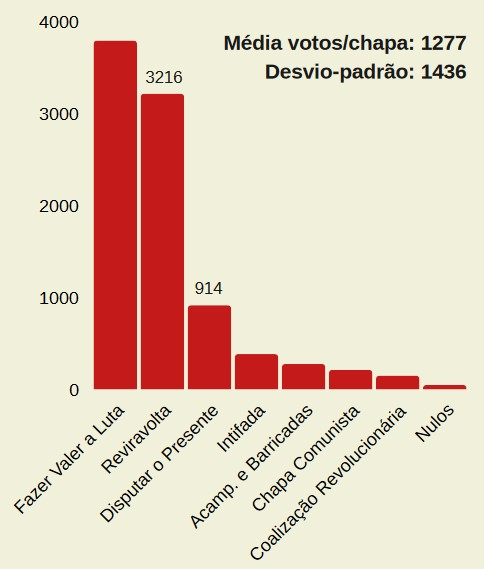
\includegraphics[width=\columnwidth]{textos//img/resultado_geral.jpg}
\end{figure}

Ainda, o resultado das eleições é utilizado na distribuição das cadeiras de representação discente nos órgãos colegiados centrais. A construção da chapa “Unidade Estudantil” é feita proporcionalmente entre as forças políticas concorrentes ao DCE Livre da USP de acordo com os votos totais obtidos na eleição da entidade. 


\subsection*{E a urna do IME?}

A urna do IME contabilizou 209 votos válidos e 1 voto nulo, e os votos ficaram distribuídos da seguinte forma: 

\begin{figure}[H]
    \centering
    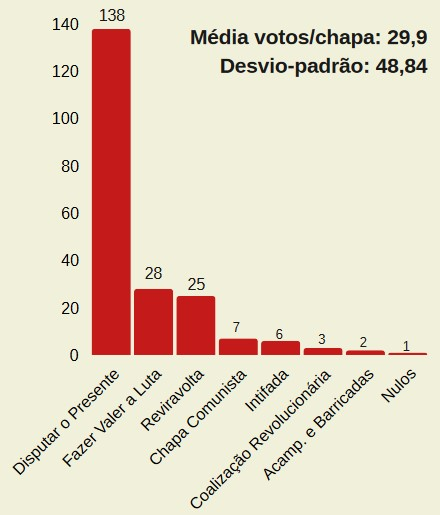
\includegraphics[width=0.88\columnwidth]{textos//img/resultado_ime.jpg}
\end{figure}


\quadradao{\normalsize}{1.2}{0}{\columnwidth}{black}{0.15cm}{
\color{black}
PARA COMPARAR
\\
ELEIÇÕES 2022 - DCE LIVRE DA USP
\\
\raggedright % alinhar à esquerda
\normalfont % para ignorar o bold
Quórum: 10.049
\\~\\
É Tudo Pra Ontem - 6.214\\
Por Todos os Cantos - 1.145\\
Nossa Voz - 1.141\\
USP Sem Medo - 825\\
Envolver - 313\\
Quebra das Correntes - 175\\
Retomada - 87\\
USP Pública, Gratuita e Para Todos - 61\\
Lula Presidente - 47\\
Nulos - 41\\
}